% Отчет по лабораторной работе №2
% Рыжиков И.С. 2022г
%=== Тип документа - статья, кегль 14пт.
\documentclass[14pt]{article}
%=== Настройка кодировок, шрифта и языка
\usepackage[utf8]{inputenc}
\usepackage{extsizes}
\usepackage[main=russian, english]{babel}
\usepackage[T2A, T1]{fontenc}
%=== Разметка документа
\usepackage{geometry} 
\geometry{
	a4paper, 
	top = 2cm,
	bottom = 2cm,
	left = 3cm,
	right = 1.5cm
}
%=== Стилизация номера страницы
\usepackage{fancyhdr}

% \pagestyle{fancy}
% \fancyhf{}
% \rfoot{\thepage}

%=== Форматирование текста
\usepackage{setspace}			% Интерлиньяж
\onehalfspacing					% 1.5 строки
\usepackage{indentfirst} 		% Красная строка с первого предложения
\setlength						% Отступ красной строки - 1.25см
	{\parindent}
	{1.25cm}	
\usepackage{titlesec}			% Форматирование заголовков
\titleformat					% Разделы
	{\section}
	[hang]
	{\normalfont\bfseries}
	{}
	{0pt}
	{}
\titlespacing
	{\section}
	{\parindent}
	{4ex}
	{0pt}
\titleformat					% Подразделы
	{\subsection}
	[hang]
	{\normalfont\itshape}
	{}
	{0pt}
	{}
\titlespacing
	{\subsection}
	{\parindent}
	{4ex}
	{0pt}

%=== Минимизируем количество переносов
\usepackage{ragged2e}
\usepackage{microtype}
\tolerance = 500
\hyphenpenalty = 20000
\emergencystretch = 1cm
%=== Таблицы
\usepackage{tabularx}	% основной тип таблиц, выравнивание по ширине
\usepackage{longtable}	% для таблиц, не вмещающихся на одну страницу
\usepackage{multirow}	% для разбиения ячеек на несколько строк
\usepackage{multicol}	% на несколько колонок
%=== ^ до этого места - минимальная преамбула документа.
%=== Далее идут опциональные, но часто использующиеся пакеты,
%=== а так же написанные мной команды, чем-то упрощающие написание отчетов
\usepackage{array}
%=== Меняем подписи к таблицам
\usepackage{caption}
\captionsetup[table]{singlelinecheck=off, justification=RaggedRight}

%=== Работа с формулами
% Набор пакетов, сильно расширяющих возможности по набору формул
\usepackage{amsmath}
% добавляет специфические для русских  статей мат. символы вроде \leqslant
\usepackage{amssymb}
% добавляет окружения для теорем и лемм	
\usepackage{amsthm}				
\usepackage{mathtools}
% номера только для тех формул, на которые есть ссылки в тексте
\mathtoolsset{showonlyrefs=true}
%=== Работа с изображениями
\usepackage{wrapfig}
\usepackage{graphicx}
\graphicspath{ {./images/} }
%=== Работа с гиперссылками
\usepackage[unicode]{hyperref}
\hypersetup{
	colorlinks=true,
	urlcolor=blue,
	filecolor=green,
	linkcolor=red
}

\begin{document}
\pagenumbering{gobble}
\clearpage
\begin{center}
	МИНОБРНАУКИ РОССИИ\\
	САНКТ-ПЕТЕРБУРГСКИЙ ГОСУДАРСТВЕННЫЙ\\
	ЭЛЕКТРОТЕХНИЧЕСКИЙ УНИВЕРСИТЕТ\\
	«ЛЭТИ» ИМ. В.И. УЛЬЯНОВА (ЛЕНИНА)\\
	Кафедра ТОЭ
	\vspace{54mm}

	ОТЧЕТ\\
	по лабораторной работе №1 \\
	Тема: «Исследование линейных резистивных систем» \\




	\vfill
	\def\arraystretch{1.5}
	\begin{tabularx}{\textwidth}{ >{\hsize=7cm}X >{\hsize=4cm}X >{\hsize=1mm}X >{\centering\arraybackslash}X }
		Студент гр. 2381 &  &  & Комосский Е.А. \\
		Студент гр. 2381 &  &  & Кузнецов И.И.  \\
		Студент гр. 2381 &  &  & Рыжиков И.С.   \\
		Преподаватель    &  &  &                \\ \cline{2-2} \cline{4-4}
	\end{tabularx}
	\def\arraystretch{1}

	\vspace{25mm}

	Санкт-Петербург\\
	2024
\end{center}
\newpage
% \pagenumbering{arabic}
% \setcounter{page}{2}

\section{Цель работы}

Экспериментальное исследование линейных разветвленных
резистивных цепей с использованием методов наложения, эквивалентного
источника и принципа взаимности.

\section{Приборы и материалы}

\begin{itemize}
    \item мультиметр;
    \item набор резисторов;
    \item соединительные провода.
    \item Схема для исследования, изображенная на рис. \ref*{fig:scheme_1}.
\end{itemize}

\begin{figure}[!h]
    \centering
    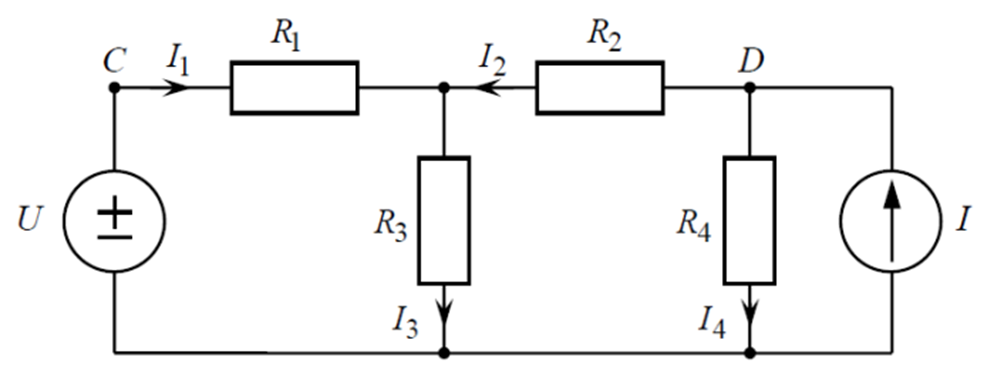
\includegraphics{scheme_1.png}
    \caption{Схема для исследования}
    \label{fig:scheme_1}
\end{figure}

$R_1 = R_2 = 1,5$ кОм, $R_3 = R_4 = 3$ кОм.

\newpage
\section{Выполнение работы}

\subsection{Исследование цепи при питании её от двух источников }

Проверим результаты эксперимента, используя уравнения Кирхгофа.
Для этого составим систему уравнений:

\begin{equation}
  \begin{cases}
    I_1 + I_2 - I_3 = 0 \\
    I - I_2 - I_4 = 0   \\
    U_1 + U_3 - U = 0   \\
  \end{cases}
\end{equation}

Подставим в уравнения значения напряжений и токов:
\begin{equation}
  \begin{cases}
    I_1 + I_2 - I_3 = 0,206 + 0,274 - 0,475 = 0,005\ (\text{мА}) \\ % OK
    I - I_2 - I_4   = 0,989 - 0,274 - 0,680 = 0,035\ (\text{мА})   \\ % Тут говно
    U_1 + U_3 - U   = 0,31 + 1,57 - 1,92    = 0,04 \ (\text{мА})       \\ % OK
  \end{cases}
\end{equation}

Учитывая погрешность измерений, можно сделать вывод, что результаты
эксперимента совпадают с результатами, полученными с помощью
уравнений Кирхгофа.



\subsection{Определение токов методом наложения}
Токи в цепи можно определить методом наложения, а именно:
ток в цепи равен алгебраической сумме токов, которые протекали бы
в цепи при включении каждого источника по отдельности.

Чтобы определить это составим таблицу, в которой будут указаны токи:

\begin{tabular}{|c|c|c|c|c|}
    \hline
    Включены источники & $I_1$, мА & $I_2$, мА & $I_3$, мА & $I_4$, мА \\
    \hline
    $U$                & $0,528$   & $-0,238$  & $0,301$   & $0,245$   \\
    \hline
    $I $               & $-0,358$  & $0,534$   & $0,138$   & $0,475$   \\
    \hline
    $U, I$             & $0,170$   & $0,296$   & $0,475$   & $0,720$   \\
    \hline
    $U, I$ (измерено)  & $0,206$   & $0,274$   & $0,439$   & $0,680$   \\
    \hline
\end{tabular}

% Пук-пук плак-плак, результаты не совпадают
\subsection{Определение тока в ветви с сопротивлением $R_3$ методом
  эквивалентного источника напряжения}

% TODO: Добавить немного букв


\subsection{Экспериментальная проверка принципа взаимности}

Принцип взаимности можно сформулировать следующим образом:

Если источник напряжение (единственный в цепи),
действуя в одной ветви линейной электрической цепи,
вызывает ток в другой ветви, то тот же источник после его
переноса во вторую ветвь вызовет в первой ветви такой же ток.

\begin{figure}[!h]
    \centering
    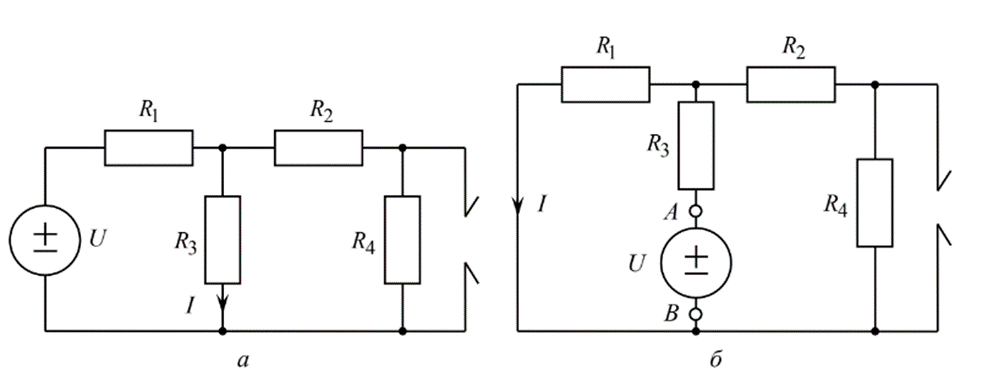
\includegraphics{reciprocity_1.png}
    \caption{Схема для проверки принципа взаимности}
\end{figure}

По результатам эксперимента $I_3=I_1^\prime$: $0,32\ \text{мА} = 0,32\ \text{мА}$.
Значит принцип подтверждается на практике.




\newpage
\section{Выводы}

В ходе выполнения лабораторной работы были изучены основные методы
анализа линейных электрических цепей: метод наложения, 
метод эквивалентного источника и принцип взаимности. 

Проведенные измерения подтвердили правильность применения уравнений Кирхгофа для анализа электрической цепи, принцип суперпозиции, принцип эквивалентного источника и принцип взаимности.

Метод наложения позволил успешно определить токи в различных ветвях цепи. Сравнение экспериментальных значений с теоретическими расчетами показало, что результаты совпадают в пределах допустимой погрешности, что подтверждает эффективность данного метода в анализе электрических цепей.

Использование эквивалентного источника напряжения для расчета тока в ветви с сопротивлением R3 также дало удовлетворительные результаты. Полученное значение тока (0,533 мА) близко к экспериментально измеренному (0,491 мА), что подтверждает правильность выбранного подхода.

Экспериментальная проверка принципа взаимности также подтвердила его справедливость: токи в разных ветвях при переносе источника напряжения остались одинаковыми (0,32 мА), что соответствует теоретическим ожиданиям.




\end{document}